%نام و نام خانوادگی:
%شماره دانشجویی: 
\مسئله{}

صورت سوال اصلی کمی نامفهوم است. فرض می‌کنیم صورت سوال اینگونه باشد: 
\newline
نحوه‌ی استفاده از مدل‌های
\lr{CRC}
در تحلیل شیٔ‌گرا را ذکر کنید.

\پاسخ{

دو استراتژی برای مدل‌سازی نیازمندی‌ها داریم\cite{pressman}:

\begin{itemize}
	\item تحلیل ساختار یافته (\lr{Structured Analysis})
	\item تحلیل شیٔ‌گرا (\lr{Object-Oriented Analysis})
\end{itemize}

در \textbf{تحلیل شیٔ‌گرا} تمرکز بر دو موضوع است: 

\begin{itemize}
	\item تعریف کلاس‌ها
	\item نحوه ارتباط و همکاری آن‌ها برای تاثیر بر نیازمندی‌های کاربر
\end{itemize}

یکی از روش‌های انجام این تحلیل استفاده از مدل‌سازی کلاس‌محور
\lr{(Class-Based Modeling)}
است. یکی از عناصر مدل‌سازی‌های کلاس‌محور، مدل‌های
\lr{CRC}
هستند. این مدل‌سازی روش ساده‌ای برای شناسایی و مدیریت کلاس‌های مربوط به سامانه یا نیازمندی‌های محصول را در اختیار ما قرار می‌دهد.


\begin{figure}[!ht]
	\centering
	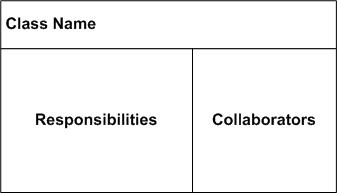
\includegraphics[scale=1.0]{figs/Q5/1.jpg}
	\caption{نحوه‌ی قرارگیری بخش‌های مختلف هر کارت
		\lr{CRC}\cite{ambler}}	
	\label{farzamfig1}
\end{figure}

امبلر
\lr{(Ambler)}
مدل‌سازی
\lr{CRC}
را اینگونه توصیف می‌کند\cite{ambler}:
\begin{latin}
A CRC model is really a collection of standard index cards that represent classes. The cards are divided into three sections. Along the top of the card you write the name of the class. In the body of the card you list the class responsibilities on the left and the collaborators on the right.
\end{latin}

برای درک بهتر این توصیف، شکل \ref{farzamfig1} را مشاهده کنید.
همچنین مثالی فرضی از یک کارت
\lr{CRC}
مربوط به دانشجو‌ها در سیستم آموزش دانشگاه را در شکل \ref{farzamfig2} مشاهده می‌کنید.

\newpage

برای تهیه‌ی یک مدل
\lr{CRC}
باید قدم‌های زیر طی شوند:

\begin{enumerate}
	\item یافتن کلاس‌ها
	\item یافتن وظایف
	\item  مشخص کردن همکاری‌ها (collaborators)
	\item نزدیک‌ چیدن کارت‌های مرتبط، هرچه ارتباط بیشتر فاصله کمتر
\end{enumerate}

\textbf{کلاس‌ها}، وظایف و همکاری‌ها را به کمک تعریف آن‌ها پیدا می‌کنیم.
هر کلاس نماینده‌ی اشیاء شبیه به یکدیگر است، هر شی‌ء می‌تواند یک شخص، مکان، چیز، رویداد یا مفهوم باشد که به مسئله یا سامانه‌ی مورد نظر مربوط است. برای مثال در یک سامانه دانشگاه، هر دانشجو یک شیء است.

\textbf{وظایف} شامل چیز‌هایی است که اشیاء یک کلاس انجام می‌دهند یا آن را می‌دانند. برای مثال برداشتن درس، یکی از وظایف کلاس دانشجو است و دانشجو شماره همراه می‌داند. دقت کنید که کلاس‌ها قادر به تغییر آنچه می‌دانند باید باشند اما قادر به تغییر آنچه کلاس‌های غیر از خودش می‌دانند نباید باشند. در مثال ذکر شده شماره همراه و برداشتن درس هر دو در قسمت وظایف کارت 
\lr{CRC}
نوشته می‌شوند.

گاهی اوقات یک کلاس وظیفه‌ای دارد که داده‌ی کافی برای انجام آن را ندارد. مثال شکل \ref{farzamfig2} را در نظر بگیرید، دانشجو در سمینار شرکت می‌کند. برای شرکت در سمینار نیازمند دانستن زمان و مکان و موضوع سمینار است یا نیاز دارد بداند که آیا سمینار همچنان ظرفیت خالی دارد یا خیر. این اطلاعات در کلاس دانشجو وجود ندارد، اما در کلاس سمینار وجود دارد. در اینجا کلاس دانشجو به \textbf{همکاری} (collaboration) با کلاس سمینار نیاز دارد تا به داده‌ی مورد نیاز دست یابد. بنابراین سمینار در قسمت همکاری‌های کارت
\lr{CRC}
دانشجو قرار دارد.



\begin{figure}
	\centering
	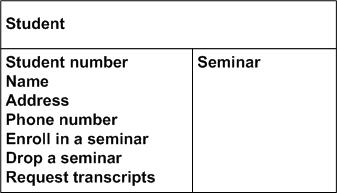
\includegraphics[scale=1.0]{figs/Q5/2.jpg}
	\caption{نمونه‌ای از کارت
		\lr{CRC}
		دانشجو‌ها در سیستم آموزش دانشگاه
		\cite{ambler}
	}	
	\label{farzamfig2}
\end{figure}


\subsection*{مراجع}

\begin{latin}
	\begingroup
	\renewcommand{\section}[2]{}%
	
\begin{thebibliography}{9}
%   Check this for adding items: https://www.student.unsw.edu.au/how-do-i-cite-electronic-sources

	\bibitem{pressman}
	R. Pressman,   B. Maxim (2014).
	S\textit{oftware Engineering: A Practitioner’s Approach, 8th Ed. }.
	McGraw-Hill.

	\bibitem{ambler}
	Ambler, Scott. (1998). The Object Primer, 3rd Ed.
	 
	
	
\end{thebibliography}
\endgroup
\end{latin}

}
